\documentclass{amsart}
\usepackage[margin=3cm]{geometry}                % See geometry.pdf to learn the layout options. There are lots.
\geometry{letterpaper}                   % ... or a4paper or a5paper or ...
%\geometry{landscape}                % Activate for for rotated page geometry
\usepackage[parfill]{parskip}    % Activate to begin paragraphs with an empty line rather than an indent
\usepackage{float}
\usepackage{graphicx}
\usepackage{amssymb}
\usepackage{epstopdf}
\usepackage{siunitx}
\usepackage{subcaption}
\usepackage{units}
\usepackage{setspace}

\DeclareGraphicsRule{.tif}{png}{.png}{`convert #1 `dirname #1`/`basename #1 .tif`.png}

\title{Speed of Light}
\author{Caspar \textsc{Lant}} % Author name

\date{\today} % Date for the report

\begin{document}

\bigskip

\maketitle % Insert the title, author and date
\begin{center}
    Intermediate Experimental Physics II\\
    \vspace{.7cm}
    \begin{tabular}{l r}
        Section: & 002\\
        \\
        Date Performed: & February 23, 2016 \\ % Date the experiment was performed
        Date Due: & March 1, 2016\\
        \\
        Partner: & Neil Saddeler\\ % Partner names
        Professor: & Prof. Andrew Kent\\
        Instructor: & David Mykytyn % Instructor/supervisor
    \end{tabular}
    \vfill
    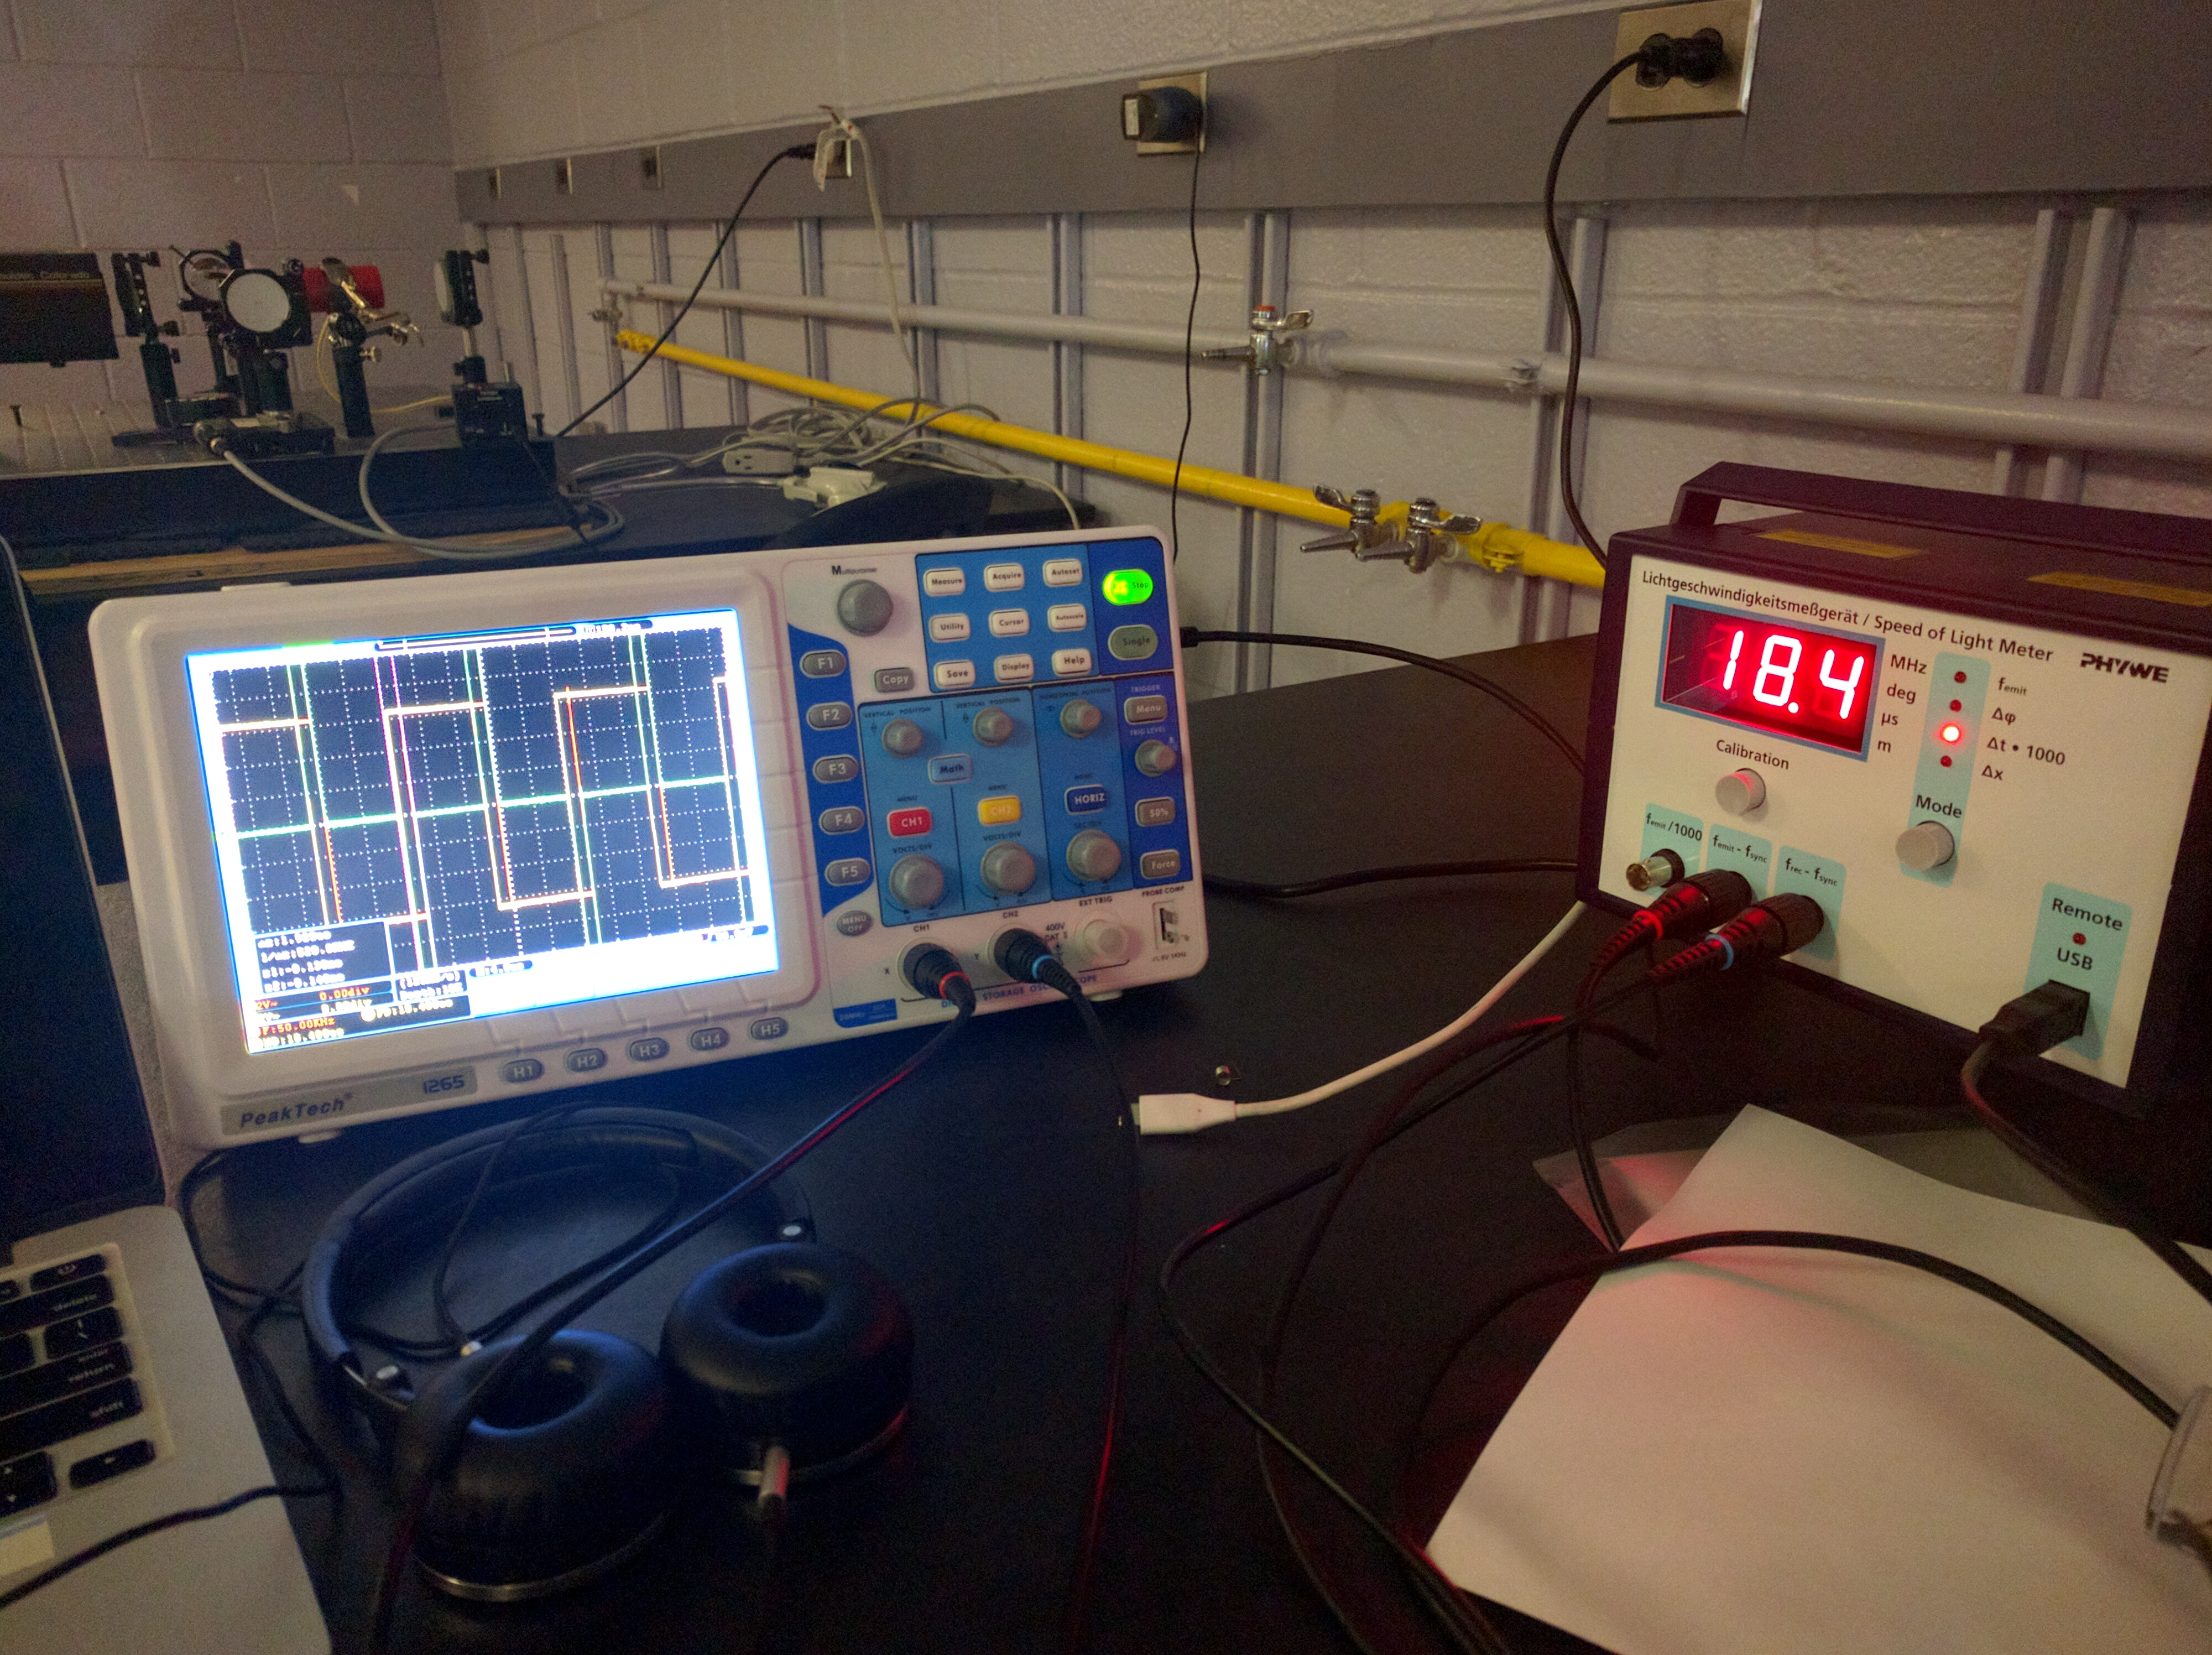
\includegraphics[width=0.8\textwidth]{Setup.jpg}
    \vfill
\end{center}

\pagebreak
\setstretch{1.5}
\paragraph{\textbf{The Objective} of this week's experiment was to arrive at a realistic value for the speed of light in air, as well as to calculate the refractive indeces of various materials under the assumption the the index of refraction of air is effectively zero.}

\section{Theoretical Background/ Abstract}
\paragraph{The speed of light in a vaccuum is a universal constant and, according to special relativity, cannot be exceeded. The speed of light is defined to be exactly $299,792,458  \ \nicefrac{m}{s}$. This value is precise because the units of meters and seconds are defined in terms of the speed of light, and not the other way around. If our understanding of the speed of light were to change somehow, or were to become more precise, humanity's standard length and time measurements would shrink or grow accordingly. At first glance, this value is mind-bogglingly large, but it turns out that it is not very difficult to measure, and as a consequence, scientists have had a good idea of the speed of light for a very long time. As I'm sure you know, we physicists often deal with times and distances that far exceed or fall hugely short of this order of magnitude. It is for this reason\-- that we can very precisely measure very small distances and times, that we are so confident in our experimentally-derived value for the speed of light in a vaccuum.\\}
\paragraph{The value of the index of refraction of a given medium is given by the ratio of the speed of light in a vaccuum to the speed of light in that medium. Obviously, this means that the index of refraction of free space is 1, and the refractive indeces of all other media is greater than one. The index of refraction of air is very close to one, and is a value that we will derive further on in this experiment.}
\begin{equation}
    n_m = \dfrac{2\Delta x+ 2l_m}{2l_m} = \dfrac{\Delta x + l_m}{l_m}
\end{equation}
Where $n_m$ is the refractive index of our medium, $\Delta x$, is the distance between the laser and the reflector, and $\l_m$ is the length of our sample medium. In these calculations, we assume that the index of refraction of air is approximately equal to one, the index of refraction in free space.
Rearranging the above definition of the index of refraction, we see that:
\begin{equation}
    c_m = \dfrac{c_a}{n_m}
\end{equation}
Where $c_m$ is the speed of light in our medium, $c_a$ is the speed of light in free space, and $n_m$ is the refractive index of our medium.

\section{Experimental Procedure}
\setstretch{1.5}
\begin{enumerate}
\item Turn on the speed of light measuring device as well as the super fancy oscilloscope.
\item Level the laser and center it on the reflector, such that it lies parallel to the measuring bar.
\item Connect the device's frequency output to one of the oscilloscope's inputs with the supplied BNC cable.
\item Verify that the frequency as reported by the oscilloscope matches the frequency of the laser.
\item Remove the cable from the device's frequncy output and link the two remaining connectors to the oscilloscope channels.
\item Move the reflector to the zero mark and set the distance reported by the measurement device to zero.
\item Move the reflector along the length of the bar to the 1 meter mark.
\item Record the value of $\Delta t$.
\item Repeat steps 7 and 8 for other positions of the reflector.
\item Now, place the water-filled tube in the path of the laser.
\item Record the length of the tube and repeat steps 5 through 9
\item Repeat steps 6 through 11 for each acrylic tube.
\item Profit.
\end{enumerate}
\setstretch{1.5}

\section{Graphs and Tables}

\begin{table}[H]
    \begin{minipage}{0.5\textwidth}
        \label{my-label}
        \begin{tabular}{c|c|c}
            $\Delta d\unit{\ (cm)} \pm 1.0$ & $\Delta t\unit{\ (\mu s)}$ & $c\unit{\ (m \times 10^8)}$ \\ \hline
            100                   & 6.96                     & 3.02                      \\
            105                   & 7.36                     & 2.99                      \\
            110                   & 7.76                     & 2.96                      \\
            115                   & 8.16                     & 2.94                      \\
            120                   & 8.48                     & 2.95                      \\
            125                   & 8.88                     & 2.93                      \\
            130                   & 9.36                     & 2.88                      \\
            135                   & 9.76                     & 2.87                      \\
            140                   & 10.32                    & 2.81                      \\
            145                   & 10.64                    & 2.82                      \\
            150                   & 10.96                    & 2.83
        \end{tabular}
    \end{minipage}
    %
    \begin{minipage}{0.2\textwidth}
    \end{minipage}
    %
    \begin{minipage}{0.3\textwidth}
        \setstretch{1.5}
        Average speed of light in air: \[\unitfrac[2.91 \times 10^8]{m}{s}\] Comparing this value to the speed of light in free space, $c = \unitfrac[2.99\times 10^8]{m}{s}$, our value for the index of refraction of air is:  \[n_a = \nicefrac{c}{c_a} = \nicefrac{2.99}{2.91} = 1.02\]
    \end{minipage}
\end{table}

The uncertainty of our measurement for the index of refraction of air is produced by our error in the distance between the reflector and the laser source. It is equal to 0.016 and is unitless. Our expected value for the index of refraction of air (which of course depends on the density of the air, which depends on the ambient temperature and pressure) is 1.00, which falls within our estimated uncertainty.

\begin{table}[H]
    \begin{minipage}{0.3\textwidth}
        \centering
        \caption{Water}
        \vspace{-0.2cm}
        $L = 51.0\ \unit{cm} \pm 0.1$
        \vspace{0.3cm}
        \label{my-label}
        \begin{tabular}{c|c}
        $d_1 \unit{\ (cm)}$ & $d_2 \unit{\ (cm)} \pm 1.5$ \\ \hline
        49.0            & 81.7                    \\
        48.5            & 84.0                    \\
        49.0            & 72.6                    \\
        48.9            & 81.1                    \\
        48.8            & 80.0                    \\
        48.4            & 87.8
        \end{tabular}
    \end{minipage}
    %
    \begin{minipage}{0.3\textwidth}
        \centering
        \caption{Acryliglas}
        \vspace{-0.2cm}
        $L = 49.0 \ \unit{cm}$
        \vspace{0.3cm}
        \label{my-label}
        \begin{tabular}{c|c}
        $d_1 \unit{\ (cm)}$        & $d_2 \unit{\ (cm)} \pm 1.5$ \\ \hline
        45.0                   & 69.6                    \\
        45.0                   & 68.6                    \\
        45.0                   & 68.5                    \\
        - & - \\
        - & - \\
        - & - \\
        \end{tabular}
    \end{minipage}
    %
    \begin{minipage}{0.3\textwidth}
        \centering
        \caption{Acrylicrap}
        \vspace{-0.2cm}
        $L = 18.3 \ \unit{cm}$
        \vspace{0.3cm}
        \label{my-label}
        \begin{tabular}{c|c}
        $d_1 \unit{\ (cm)}$            & $d_2 \unit{\ (cm)} \pm 1.5$ \\ \hline
        13.9                       & 37.3                    \\
        13.9                       & 34.0                    \\
        13.9                       & 39.2                    \\
        13.9                       & 37.5                    \\
        13.9                       & 35.6                    \\
        13.9                       & 37.2
        \end{tabular}
    \end{minipage}
\end{table}

%
% \begin{figure}
%     \begin{minipage}{.45\textwidth}
%         \includegraphics[width=\textwidth]{path}
%         \caption
%     \end{minipage}
%     %
%     \begin{minipage}{.45\textwidth}
%
%     \end{minipage}
% \end{figure}
\section{Questions}

\begin{enumerate}
\item {\textit{Why doe the speed of light in the different mediums?}
\begin{quote}
I'm guessing that this question should read ``Why does the speed of light change in the different media?", the answer to which is that different media have different densities and other material properties, which have the effect of obstructing light.
\end{quote}}

\item{\textit{Does the wavelength of the light change in different mediums?}
\begin{quote}
    Yup, but not the frequency. We know that the energy carries by a photon in a beam of light is given by its freuency times the Planck constant: $E = h\nu$, and does not change between material boundaries. The speed of light, like other waves, is equal to its frequency times its wavelength: $v = \lambda f$. We know that the speed of light changes between media, and that the frequency of light is fixed, so its wavelength must change.
\end{quote}}

\item{\textit{How does the intensity of the light vary in the different materials?}
\begin{quote}
    $I = \dfrac{cn\epsilon_0}{2}E^2$, so the intensity of light increases with the refractive index of the medium it travels in.
\end{quote}}

\end{enumerate}

\section{Analysis}
The uncertainty of our measurement for the index of refraction of air is produced by our error in the distance between the reflector and the laser source. It is equal to 0.016 and is unitless. Our expected value for the index of refraction of air (which of course depends on the density of the air, which depends on the ambient temperature and pressure) is 1.00, which falls within our estimated uncertainty. \\
The speed of light in our first medium, $\text{H}_2\text{O}$ is slightly higher than expected, producting an index of refraction value of $1.39$. The expected value for the refractive index of water is 1.33, but of course this value is dependent on temperatue, a quantity that we did not measure. However, the water was fairly cold, which is consistent with the increased index of refraction that we observed. Another factor that likely contributed to this high index of refraction was the fact that our water was contained in a tube bounded by two glass discs. The assumption was that we could ignore them because their thickness was substantially smalled than the length of water that the laser passed through, but because the index of refraction of glass is likely higher than that for water, their presence would likely increase the value of our measurement.\\
The index of refraction of our second medium, ``acryliglas", was reported to 1.49. This is consistent with values that I found on line, but is likely a bit high given our assumption that the index of refraction of air was one.\\
The index of refraction of our third medium was 2.25, which is much higher than one would expect for acrylic, but the rod was reportedly full of impurities, which would have the effect of increasing the measured refractive index.



\end{document}
